\documentclass[10pt,a4paper]{article}
\usepackage[utf8]{inputenc}
\usepackage[italian]{babel}
\usepackage{amsmath}
\usepackage{amsfonts}
\usepackage{amssymb}
\usepackage{graphicx}
\usepackage{siunitx}
\usepackage[left=2cm,right=2cm,top=2cm,bottom=2cm]{geometry}
\newcommand{\rem}[1]{[\emph{#1}]}
\newcommand{\exn}{\phantom{xxx}}

\author{Gruppo 1.BN \\ Massimo Bilancioni, Alessandro Foligno, Giuseppe Zanichelli }
\title{Amplificatore a transistor}


\begin{document}

\date{31 ottobre 2018}
\maketitle
\section{montaggio del circuito e verifica del punto di lavoro}

Le misure dei componenti tramite multimetro :

$ R_1 = (178.2\pm 1.4)\si{\kilo\ohm}$, $ R_2 = (19.20\pm 0.15)\si{\kilo\ohm}$, $ R_C = (9.99\pm 0.08)\si{\kilo\ohm}$, $ R_E = (0.986\pm 0.008)\si{\kilo\ohm}$,

 $ C_{IN} = (216 \pm 9)\si{\nano\farad}$, $ C_{OUT} = (105\pm 4)\si{\nano\farad}$

Infine la tensione del generatore è  $V_{CC} = (20.7\pm 0.1)\si{\volt}$.


a) La tensione  di lavoro risulta  $V_{CE}^Q = (7.41 \pm 0.04) \si{\volt}$ e  la corrente di collettore (misurata come caduta di d.d.p. ai capi di $R_C$) è $I_C^Q = (1.22\pm 0.01) \si{\milli\ampere}$. 
Teoricamente ci si aspetta  $V_{CE}^Q + I_C^Q(R_C+ R_E)= V_{CC}$  (si è assunto $I_C^Q \simeq I_E^Q$, l'errore derivante  da questa approssimazione è dell' $1 \%$ se si considera un guadagno in continua attorno a $100$ )
; inserendo i valori, la parte a destra dell'equazione è uguale a $(20.8\pm 0.2)\si{\volt}$ che è compatibile con il valore di $V_{CC}$.

Se è vero che  $I_B \ll$ della corrente che scorre nel ramo di $R_2$, allora vale $I_C^Q \simeq (V_{BB}-V_{BE})/R_E$ dove            

$V_{BB}= V_{CC}/(1+ R_1/R_2)$, ma $(V_{BB}-V_{BE})/R_E= 1.41 \si{\milli\ampere}$ ed essendo tutti gli errori intorno all' $1\%$ è incompatibile con il valore misurato di $I_C^Q$; questo significa che non è vera l'approssimazione sopra.


b) Le tensioni misurate sono $V_B = (1.82\pm 0.01)\si{\volt}$,  $V_E = (1.21\pm 0.01)\si{\volt}$,  $V_{BE} = (0.61\pm 0.01)\si{\volt}$, 

 $V_C = (8.61\pm 0.05)\si{\volt}$.

c) Dal datasheet del transistor il valore di $h_{FE}$ per il nostro punto di lavoro dovrebbe essere compreso tra 80 e 130.

Segue che il valore della corrente di base dovrebbe essere compreso tra $0.009\si{\milli\ampere} < I_B< 0.015\si{\milli\ampere} $.

Le correnti che scorrono nei rami di $R_1$, $R_2$ sono rispettivamente $I_{R_1} = (V_{CC}-V_{B})/R_1 = (0.106\pm 0.002)\si{\milli\ampere}  $, $I_{R_2} = V_{B}/R_2=(0.095\pm 0.001)\si{\milli\ampere} $ .

Dalla differenza si ottiene $I_B = (0.011\pm 0.002) \si{\milli\ampere} $ che è circa 10 volte inferiore alla corrente che scorre nel partitore.

Continuando la parte finale del punto a), questo si traduce nel fatto che nel calcolo di $V_{BB}$ al posto di $R_2 $ andrebbe messa la resistenza equivalente che è più piccola di circa il $10\%$. Questo comporta un errore del $10\% $ sul calcolo di $V_{BB}\simeq 2\si{\volt}$ che a questo punto diventa compatibile con $V_{B}$ misurato.



\section{Risposta a segnali sinusoidali di frequenza fissa}

Abbiamo scelto una frequenza di lavoro intorno ai $7.40$ \si{\kilo\hertz}.

a) 
\vspace{0.5cm}

i)  Abbiamo verificato l'inversione di fase per VOUT, la figura sotto riporta quanto osservato.

\begin{figure}[h]
	\centering
	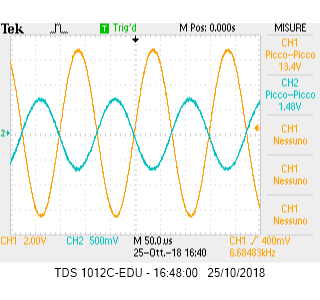
\includegraphics[scale=0.5]{oscilloscopio.png}

	
	
\end{figure}

ii)  Facendo una media dei guadagni per piccole  ampiezze diverse di VIN, otteniamo :\[A_v= (9.76\pm0.01) \]
  (VIN e VOUT sono stati misurati sui due canali differenti dell'oscilloscopio,per questo abbiamo considerato gli errori scorrelati)

Il valore atteso per il guadagno è $A_{v,att} \simeq \frac{R_C}{R_E}= 10.1\pm 0.1$
\begin{table}[h]
	\centering
	\begin{tabular}{|c|c|c|}
		\hline 
		 VIN (\si{\volt}) &  VOUT (\si{\volt})   & VOUT/VIN\\
		\hline 
	$0.228 \pm  0.06 $& $2.20\pm 0.06$& $9.65 \pm 0.04$\\
	$0.320\pm 0.08 $& $3.12 \pm 0.08$& $9.75 \pm0.04$\\
	$0.528\pm 0.015 $& $5.14 \pm 0.15$& $9.73\pm 0.04$ \\
	$0.752\pm 0.021$& $7.32\pm 0.21$ & $9.73\pm 0.04$\\
	$1.02\pm 0.03 $& $10.2\pm 0.3$& $10\pm 0.04 $\\
	$1.27\pm 0.04$ & $12.3\pm 0.4 $& $9.69\pm 0.04 $\\

		\hline 
	\end{tabular} 
\end{table}

\begin{figure}[h]
	\centering
	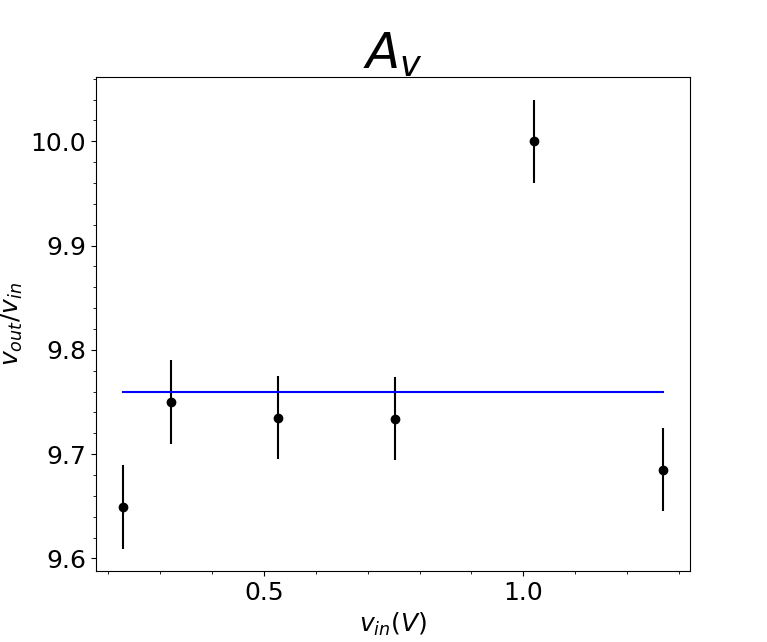
\includegraphics[scale=0.45]{guadagno.png}

	
	
\end{figure}

iii) Prima degli 1.3 \si{\volt}pp come si vede dalla tabella l'amplificazione del segnale è entro i limiti lineare,  per un segnale in ingresso di circa $1.60$ \si{\volt}pp si iniziano a vedere distorsioni per VOUT, in particolare si nota inizialmente clipping inferiore, mentre per tensioni ancora superiori si vede un clipping superiore.

iv) Nella figura si vede il clipping inferiore; è dovuto al fatto che il transistor passa dal regime attivo al regime di saturazione, e questo accade perchè quando $v_{in}$ è massimo e la sua ampiezza sufficientemente grande $ V_{CB}$ diventa negativo.
In questo regime $|V_{CE}|\ll  V_{CC}$, quindi $ I_C \simeq V_{CC}/(R_E+R_C)$ e  se chiamo $V_{out,min}$ il valore a cui viene tagliato il segnale vale \[V_{out,min} -V_C= - I_C R_C = - V_{CC}\frac{R_C}{R_E+R_C}\]
da cui 
$V_{out,min} = -(6.74\pm 0.14) \si{\volt}$; questo valore non torna con il valore misurato, che è $V_{out,clip} = -(8.5\pm 0.2) \si{\volt}$.

Ci si aspetta anche una distorsione per i picchi superiori di $V_{out}$ (il clipping superiore osservato), infatti nel caso   $V_{in}$ abbia un'ampiezza grande, quando è minimo può far assumere a  $V_{B}$ valori negatvi e portare così il transistor in interdizione.
Il segnale con clipping è asimmetrico, dato che il passaggio alla zona di interdizione per il clipping superiore avviene per segnali in ingresso più ampi rispetto al clipping inferiore, che quindi si manifesta prima.

\begin{figure}[h]
	\centering
	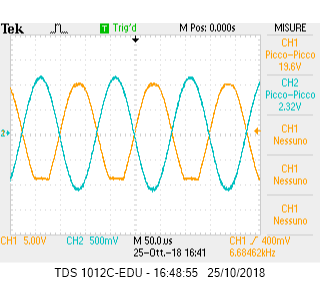
\includegraphics[scale=0.5]{clipping.png}
	\label{Clipping osservato (inferiore e superiore)}
\end{figure}
\section{Diagramma di Bode}
 Campionando in un intervallo di frequenze che spazia da 1\si{\hertz} a 1\si{\kilo\hertz}, abbiamo costruito un diagramma di Bode del guadagno. I punti sperimentali sono riportati in seguito.
 \begin{figure}[h]
 	\centering
 	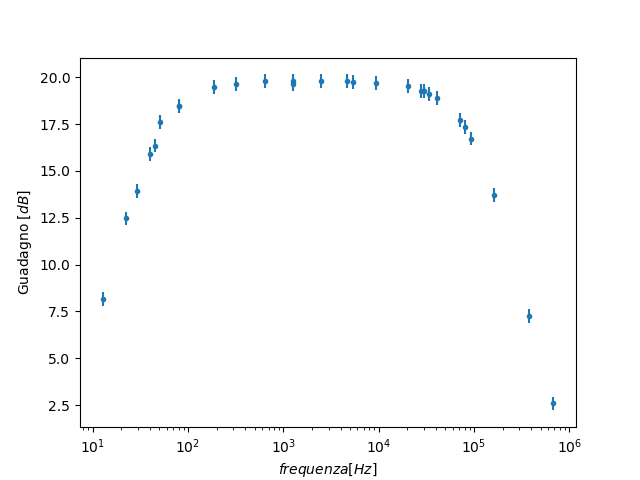
\includegraphics[scale=0.5]{dataBodeplot.png}
	
	
\end{figure}
Visivamente l'andamento sembra quello tipico di un passabanda, eppure, oltre alla traslazione del guadagno massimo (che in questo caso è $> 1$, grazie al transistor), l'andamento asintotico ai due estremi non è di $\pm 20 dB/Decade$, come nel caso di passa basso e alto in cascata, bensì di circa $-15 \pm0.3dB/Decade $ per basse frequenze e $ 17.7\pm0.2 dB/Decade$ per alte frequenze.
Questi numeri sono ottenuti da fit lineari nelle tre regioni:
\begin{figure}[h]
	\centering
	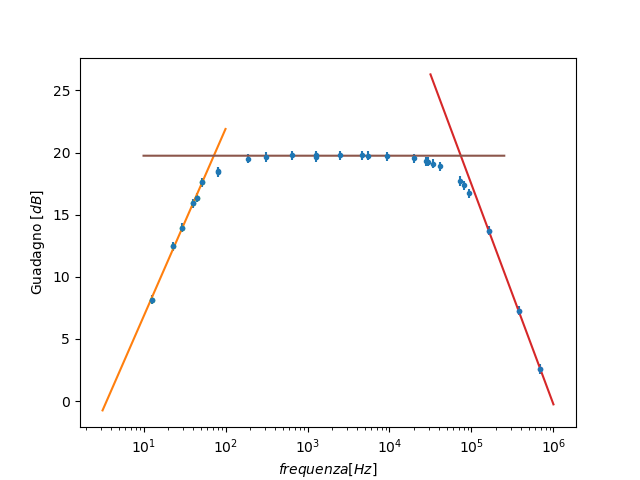
\includegraphics[scale=1]{fit.png}
	\caption{fit del passa banda}
\end{figure}
Lo smorzamento per basse frequenze lo riteniamo dovuto sostanzialmente all'effetto di $C_{IN}$ che si comporta come un passa alto. Trascuro l'effetto di $C_{OUT}$, dato che $|Z_{oscilloscopio}|\approx1 M\Omega$, la frequenza di taglio associata a questo passa-alto è $f_t = 1 /(2\pi R_{oscill} C_{out}) \simeq 1.7 \si{\hertz}$.
La funzione di trasferimento del passa-alto  è del tipo:\[A=\frac{1}{\sqrt{1+(f_t/f)^2}}\] con $f_t=1/(2\pi R_{eq} C_{IN})$ e  nell'approssimazione in cui l'impedenza dei rami del collettore ed emettitore sia molto più grande di $R_2$, posso considerare il passa-alto e il transistor in cascata e quindi $R_{eq} \sim R_2$ per cui si ottiene $ f_t \sim 40 \si{\hertz}$.

Tuttavia l'andamento che segue la curva  non è esattamente, come preannunciato, quello atteso. La pendenza minoreper basse frequenze  potrebbe  essere spiegata  con un aumento del guadagno del transistor. 
Viceversa supponiamo che,ad  alte frequenze, l'andamento da passa basso sia dovuto agli effetti induttivi non trascurabili del circuito, ed in particolare della basetta.
Lo smorzamento, di nuovo non è esattamente di $-20 dB/Decade$, supponiamo, di nuovo, a causa del comportamento non lineare del transistor.

\section*{Dichiarazione}
I firmatari di questa relazione dichiarano che il contenuto della relazione \`e originale, con misure effettuate dai membri del gruppo, e che tutti i firmatari hanno contribuito alla elaborazione della relazione stessa.

\end{document}